\documentclass[../thesis.tex]{subfiles}

\begin{document}

\section{Introduction}

%%%  Introduce for Autonomous Driving : Motivation %%%
% The rapid urbanization globally in the recent past has led to severe road congestion, rise in pollution levels and an increase in road accidents, therefore presenting a very grim picture of the current state of urban transportation. At the moment, private automobiles are widely recognized as an unsustainable solution for the future of personal urban mobility \cite{reinventing}. Fortunately however, great strides have been made in the development of autonomous driving technologies, energized by the successful demonstrations by some teams at the DARPA Urban Challenge \cite{boss, multimodaltartan}. While offering an opportunity to develop sustainable and safe solutions to personal mobility \cite{usecases_of_AD}, they also hint at a complete overhaul of the urban transportation landscape by ushering in Autonomous Vehicles-on-Demand. 

%%%  Introduce for Autonomous Driving : Alternative learning-based approach %%%
One of the key challenges to building accurate and robust autonomous navigation systems is to develop a strong intelligence pipeline that is able to efficiently gather incoming sensor data and take suitable control actions with good repeatability and fault-tolerance. In the past, this was addressed in a modular fashion, where  specialized algorithms were developed for each sub-system and later integrated with some fine tuning. More recently however, there is great interest in applying a more end-to-end approach wherein one can learn a complex mapping that goes directly from the input to the output by leveraging the availability to a large volume of task specific data. This approach is purported to perform better since we are optimizing the whole system. 
% \todo{mention why this is better}

%%% Introduce Deep Learning and Deep Reinforcement Learning : Motivation on true AI for decision making %%%%%%%%

This end-to-end approach has now become a viable alternative thanks to the extension of deep learning's success to robotics and has been applied successfully to autonomous driving \cite{deepdriving,nvidiacar,endtoendcars}. 
% in diverse domains like speech recognition\cite{graves2013speech,hinton2012deep}\todo{someone remove these?}, computer vision\cite{krizhevsky2012imagenet,simonyan2014very}, and 
However, the traditional deep supervised learning-based driving requires labeling and may not be able to deal with the problem of accumulating errors \cite{ross2011reduction}. On the other hand, deep reinforcement learning (DRL) provides a much better formulation that allows policy improvement with feedback, and has been shown to achieve human-level performance on many gaming environments \cite{mnih2013playing, mnih2015human,2016-TOG-deepRL}.

%%% Motivation of this work: Multi-modal Perception, Multi-modal Deep learning %%%%%%%%
Previous work in DRL predominantly learned policies based on a single input modality, i.e., either low-dimensional physical states, or high-dimensional pixels. For autonomous driving task where enhancing safety and accuracy to the maximum extent possible is emphasized, developing policies that operate with multiple inputs is crucial. Indeed, multi-modal perception was an integral part of autonomous navigation solutions and even played a critical role in their success \cite{multimodaltartan} before the advent of end-to-end deep learning based approaches. Sensor fusion offers several advantages namely robustness to individual sensor noise/failure, improved object classification and tracking \cite{elfring2016multisensor, cho2014multi, darms2008classification}, robustness to varying weather and environmental conditions, etc. 
% Previous work in DRL predominantly learned policies based on a single input modality, i.e., either low-dimensional physical states, or high-dimensional pixels. We have to however keep in mind the importance of enhancing safety and accuracy to the maximum extent possible in autonomous driving. In this light, we believe that it is worth exploring tangible ways to develop policies that operate with multiple inputs. 

Recently, there is also an great progress on extending DRL approaches to multi-input fashion in order to tackle complex robotics tasks such as human-robot-interaction \cite{qureshi2016robot} and manipulation \cite{levine2016end}. Recently, \citet{mirowski2017a} proposed an novel approach namely \textit{NAV A3C} and embedded information such as vision, depth, and agent velocity for maze navigation. However, it is worth mentioned that the system dynamic is relatively simple compared with autonomous driving.
% Multi-modal perception was an integral part of autonomous navigation solutions and even played a critical role in their success \cite{multimodaltartan} before the advent of end-to-end deep learning based approaches. Sensor fusion offers several advantages namely robustness to individual sensor noise/failure, improved object classification and tracking \cite{elfring2016multisensor, cho2014multi, darms2008classification}, robustness to varying weather and environmental conditions, etc. Multi-modal deep learning, in general, is an active area of research in other domains like audiovisual systems \cite{ngmultimodal}, gesture recognition \cite{moddrop}, text/speech and language models \cite{languagemultimodal,srivastava2012multimodal}, etc. However, Multi-modal learning is conspicuous by its absence in the modern end-to-end autonomous navigation literature. 

%%% Brief summary of the contribution of this work  %%%%%%%%
In this work, we present an end-to-end controller that uses multi-sensor input to learn an autonomous navigation policy in a physics-based gaming environment called TORCS \cite{wymann2000torcs}. To show the effectiveness of Multi-modal Perception, we picked two popular continuous action DRL algorithms namely Normalized Advantage Function (NAF) \cite{CDQN} and Deep Deterministic Policy Gradient (DDPG) \cite{DBLP:journals/corr/LillicrapHPHETS15}, and augmented them to accept multi-modal input. We limit our objective to only achieving autonomous navigation without any obstacles or other cars. This problem is kept simpler deliberately to focus our attention more on analyzing the performance of the proposed multi-modal configurations using extensive quantitative and qualitative testing. We believe however that it is representative of the larger urban navigation problem, and we ensure that our proposed network architecture is task-agnostic and transferable. We show through extensive empirical testing that a multi-modal deep reinforcement learning architecture achieves higher average reward.
% \todo{add more details about results}

Moreover, we also observe that while a multi-modal policy greatly improves the reward, it might rely heavily on all the inputs to the extent that it may fail completely even if a single sensor broke down fully or partially. This undesirable consequence renders sensor redundancy useless. To ensure that the learned policy does not succumb to such over-fitting, we apply a novel stochastic regularization method called \emph{Sensor Dropout} during training. 

%%% Intro : Summarize different current approaches Dropout, DropConnect, ModDrop, Zoneout, Blockout, Modout, etc. %%%
Stochastic regularization is an active area of research in deep learning made popular by the succes of, \textit{Dropout} \cite{dropout}. Following this landmark paper, numerous extensions were proposed  to further generalize this idea such as \textit{Blockout} \cite{blockout}, \textit{DropConnect} \cite{dropconnect}, \textit{Zoneout} \cite{zoneout}, etc. In the similar vein, two interesting techniques have been proposed for specialized regularization in the multi-modal setting namely ModDrop \cite{moddrop} and ModOut \cite{modout}. Given a much wider set of sensors to choose from, ModOut attempts to identify which sensors are actually needed to fully observe the system behavior. This is out of the scope of this work. Here, we assume that all the sensors are critical and we only focus on improving the state information based on inputs from multiple observers. ModDrop is much closer in spirit to the proposed \emph{Sensor Dropout (SD)}. However, unlike ModDrop, pretraining with individual sensor inputs using separate loss functions is not required. A network can be directly constructed in an end-to-end fashion and \emph{Sensor Dropout} can be directly applied at the sensor fusion layer just like Dropout. Its appeal lies in its simplicity during implementation and is designed to be applicable even to the DRL setting. As far as we know, this is the first attempt at applying stochastic regularization in a DRL setting. We show extensive simulation results to validate the net improvement in performance and robustness with Sensor Dropout. 

Through extensive empirical testing we show the following exciting results in this paper:
\begin{enumerate}
\item Multimodal-DRL with Sensor Dropout (SD) reduces performance drop in a noisy environment from $\approx 30\%$ to just $5\%$, when compared to a baseline single sensor system.
\item Policies learned using SD best leverage the multi-modal setting by greatly reducing over-dependence on any one sensing modality. Additionally, for each sensor it was observed that SD enforces sparsity and promotes each sensor to base the policy primarily on intuitive and salient features.
\item A multi-modal policy with SD guarantees functionality even in a face a sensor failure. This is a huge plus and the best use-case for the need for redundancy in safety-critical application like autonomous navigation.
\end{enumerate}
% \todo{come back and carefully review this last para after the finishing the paper. Highlight some key results here to grab attention} 
%%% Paper Summary %%%

% The report is organized as follows. Section 2 summarizes the background and two DRL algorithms we extended in this work. Section 3 introduces Multi-modal network architecture, and propose a new stochastic regularization technique called \emph{Sensor Dropout}. The performance of Sensor Dropout is then validated in Section 4, with the problem setup in the TORCS simulator, and other testing results. In Section 5, we summarize our results and discuss key insights obtained through this exercise. Finally, Section 6 contains conclusions and ideas for future work. 

\section{Background}
\subsection{Deep Reinforcement Learning (DRL)}

%% general introduction of RL notation and several useful function (Q, V, A, mu, ...) %%%

We consider a standard Reinforcement Learning (RL) setup, where an agent operates in an environment ${E}$. At each discrete time step $t$, the agent observes a state $s_t \in \mathcal{S}$, picks an action $a_t \in \mathcal{A}$, and receives a scalar reward $r(s_t, a_t) \in \mathbb{R}$ from the environment. The return $R_t = \sum^T_{i=t} \gamma^{(i-t)}r(s_i,a_i)$ is defined as total discounted future reward at time step $t$, with $\gamma$ being a discount factor $\in [0,1]$. The objective of the agent is to learn a policy that eventually maximizes the expected return.
% as show below:  \todo{add a max to the equation below. The equation below needs review or consider omitting it}
% \begin{align}
% \centering
% J = \mathbb{E}_{s_i, r_i \sim E~, a_i \sim \pi}[R_1] \label{equ:obj-func} 
% \end{align}
% $\pi$ denotes the learned policy, defined as any function that maps a given state to a suitable action, and 
The learned policy, $\pi$, can be formulated as either stochastic $\pi(a|s) = \mathbb{P}(a|s)$, or deterministic $a = \mu(s)$. The value function $V^{\pi}$ and action-value function $Q^{\pi}$ describe the expected return for each state and state-action pair upon following a policy $\pi$. \begin{align}
V^\pi(s_t) &= \mathbb{E}_{r_{i \geq t}, s_{i > t} \sim E, a_{i \geq t} \sim \pi} [R_t | a_t, s_t] \\
Q^\pi(s_t, a_t) &= \mathbb{E}_{r_{i \geq t}, s_{i > t} \sim E} [r(s_t, a_t) \nonumber \\
&\qquad + \gamma \mathbb{E}_{a_{i > t} \sim \pi} [Q^\pi(s_{t+1}, a_{t+1})]]
\end{align}
Finally, an advantage function $A^{\pi}(s_t,a_t)$ is defined as the additional reward or advantage that the agent will have for executing some action $a_t$ at state $s_t$ and its is given by $A^{\pi}(s_t,a_t) = Q^\pi(s_t, a_t) - V^\pi(s_t)$. 

%% Deep architecture on RL -> DRL! %%%
In high dimensional state/action space, these functions are usually approximated by a suitable parametrization. Accordingly, we define $\theta^Q$, $\theta^V$, $\theta^A$, $\theta^\pi$, and $\theta^\mu$ as the parameters for approximating $Q$, $V$, $A$, $\pi$, and $\mu$ functions, respectively. It was generally believed that using non-linear function approximators for both $Q$ and $V$ functions would lead to unstable learning in practice. Recently, \citet{mnih2013playing} applied two novel modifications, namely \textit{replay buffer} and \textit{target network}, to stabilize the learning with deep nets. Later, several variants were introduced that exploited deep architectures and extended to learning tasks with continuous actions \cite{DBLP:journals/corr/LillicrapHPHETS15,A3C,CDQN,TRPO}. 

To exhaustively analyze the effect of multi-sensor input and the new stochastic regularization technique, we picked two algorithms in this work namely DDPG and NAF. It is worth noting that the two algorithms are very different, with DDPG being an off-policy actor-critic method and NAF an off-policy value-based one. By augmenting these two algorithms, we highlight that any DRL algorithm, modified appropriately, can benefit from using multiple inputs. Before introducing the multi-modal architecture, we briefly summarize the two algorithms below.
% followed by proper regularization technique, as a \textit{front-end} sensor-fusion method is generalized to most \textit{back-end} DRL algorithms for joint optimization.


\subsection{Normalized Advantage Function (NAF)} 
\label{sec:CDQN}

%%% Q-learning %%%
Q-learning \cite{sutton1999policy} is an off-policy model-free algorithm, where agent learns an approximated $Q$ function, and follows a greedy policy $\mu(s)=\arg\max_aQ(s,a)$ at each step. The objective function 
% (\ref{equ:obj-func}) 
$J = \mathbb{E}_{s_i, r_i \sim E~, a_i \sim \pi}[R_1]$, can be reached by minimizing the square loss Bellman error $L = \frac{1}{N} \sum_i^N (y_i-Q(s_i,a_i|\theta^Q))^2$,
% \begin{align}
% \centering
% L = \frac{1}{N} \sum_i^N (y_i-Q(s_i,a_i|\theta^Q))^2
% \end{align}
where target $y_i$ is defined as $r(s_i,a_i) + \gamma Q(s_{i+1},\mu(s_{i+1}))$.

%%% DQN and C-DQN %%%

% Deep Q-Network(DQN) parametrized $Q$ function with deep architecture\cite{mnih2013playing}, and has been shown to emulate human performance \cite{mnih2015human} in many Atari games using just image pixels as input. However, in all of these games, action choices are limited and discrete. 
Recently, \citet{CDQN} proposed a continuous variant of Deep Q-Learning by a clever network construction. The $Q$ network, which they called Normalized Advantage Function (NAF), parameterized the advantage function quadratically over the action space, and is weighted by non-linear feature of states. 
\begin{align}
\centering
Q(s,a|\theta^Q) &= A(s,a | \theta^\mu, \theta^L) + V(s|\theta^V) \\
A(s,a | \theta^\mu, \theta^L) &= -\frac{1}{2}(a-\mu(s|\theta^\mu))^T P(s|\theta^L)\nonumber \\
&\qquad \qquad \qquad(a-\mu(s|\theta^\mu)) \label{equ:NAF} \\
P(s|\theta^L) &= L(s|\theta^L)^TL(s|\theta^L) \label{equ:P}
\end{align}
During run-time, the greedy policy can be performed by simply taking the output of sub-network $a = \mu(s|\theta^\mu)$. The data flow at forward prediction and back-propagation steps are shown in Fig. \ref{fig:CDQN-DDPG} (a) and (b), respectively.

\begin{figure}[t]
\begin{center}
\centerline{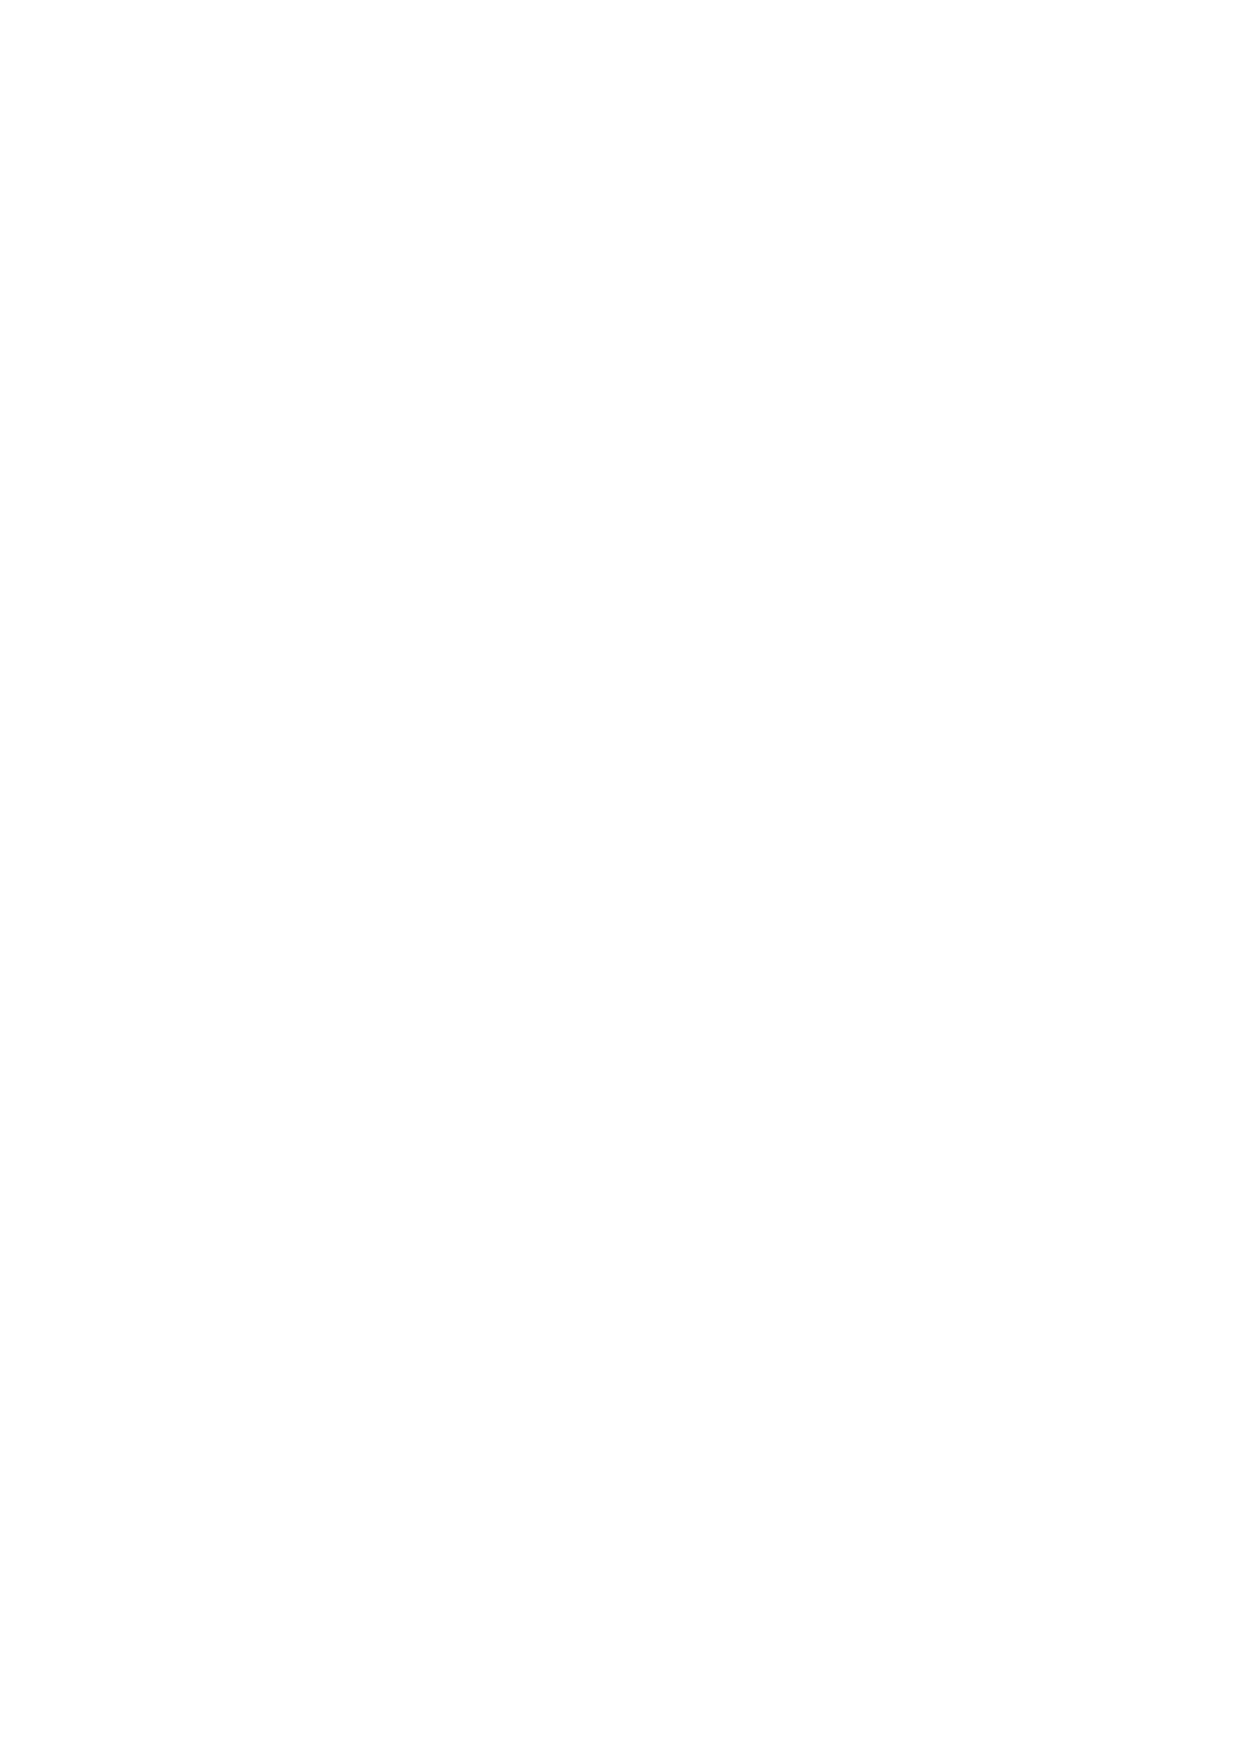
\includegraphics[width=\columnwidth,trim= 80 900 110 70, clip=true]{./MultimodalDRL/fig/naf_ddpg}}
\caption{Schematic illustration of (a) forward and (b) back-propagation for NAF, and (c) forward and (d) back-propagation for DDPG. Green modules are functions approximated with Deep Nets.}
\label{fig:CDQN-DDPG}
\end{center}
\end{figure} 

\subsection{Deep Deterministic Policy Gradient (DDPG)}
%%% Actor-Critic and DPG %%%
An alternative approach to continuous RL tasks was the use of an actor-critic framework, which maintains an explicit policy function, called \textit{actor}, and an action-value function called as \textit{critic}. 
% Among many other variants, we limited our discussion on a recently popular\todo{} algorithm called Deep Deterministic Policy Gradient (DDPG). 
In \citet{dpg}, a novel \emph{deterministic} policy gradient (DPG) approach was proposed and it was shown that deterministic policy gradients have a model-free form and follow the gradient of the action-value function. 
\begin{equation}
\nabla_{\theta^\mu} J = \mathbb{E}[\nabla_a Q(s,a|\theta^Q) \nabla_a \mu(s)]
\label{dpg}
\end{equation}
\citet{dpg} proved that using the policy gradient calculated in (\ref{dpg}) to update model parameters leads to the maximum expected reward.
% From the practical standpoint, this modification had huge implications. In the stochastic case, the policy gradient integrates over state-action space, whereas in the deterministic case it only integrates over the state space. As a result, computing the deterministic policy gradient requires fewer samples.

%%% DDPG %%%
Building on this result, \citet{DBLP:journals/corr/LillicrapHPHETS15} proposed an extension of DPG with deep architecture to generalize their prior success with discrete action spaces \cite{mnih2015human} onto continuous spaces. Using the DPG, an off-policy algorithm was developed to estimate the $Q$ function using a differentiable function approximator. Similar techniques as in \cite{mnih2015human} were utilized for stable learning. In order to explore the full state and action space, an exploration policy was constructed by adding Ornstein-Uhlenbeck noise process \cite{uhlenbeck1930theory}.
% In short, actions are chosen stochastically but a deterministic policy gradient is learned. 
The data flow for prediction and back-propagation steps are shown in Fig. \ref{fig:CDQN-DDPG} (c) and (d), respectively.

\section{Multimodal Deep Reinforcement Learning}

% \subsection{Motivation} 
Multimodal DRL aims to leverage the availability of multiple, potentially imperfect, sensor inputs to improve learned policy. 
% This problem is critical as a further step toward the real-world robotics application given the current state-of-the-art DRL agents on many realistic simulators. 
Most autonomous driving vehicles have been equipped with an array of sensors like GPS, Lidar, Camera, and Odometer, etc \cite{hudda2013self}.
% While there exist some previous work on Sensor-Fusion for autonomous driving, it has not been extended so far - to the best of our knowledge - to Deep Learning based end-to-end approaches. 
% Currently, the most promising demonstration of an effective end-to-end framework for autonomous driving is from NVIDIA \cite{nvidiacar}. While this work has some form of sensor fusion, it should be noted that they fuse information from the \textit{same} type of sensor (cameras in this case) but placed in different, but strategic, locations on the car. We argue that a more robust strategy for sensor-fusion is to obtain information from different type of sensors. 
While one would offer a long range noisy estimate, the other would offer a shorter range accurate one. When combined though, the resulting observer will have a good and reliable estimate of the environment. 
% It is important to note that some of these sensors, like GPS and odometers, are readily available but unfortunately seldom included in these models. 
% Another key deviation in this work is the choice of DRL over the more tried and tested waters of Supervised Learning. We justify this migration in the interest of better generalization and allowing for a more exploration-friendly setting. Recently, there have been a great demands and improvements on realistic simulator \cite{deepdrive,udacity} with the hope that the acquired learning in such a simulator can be transferable to the real world with minimal tuning. We are inspired by this new development that provides the potential to work around the large sampling requirements of DRL algorithms, and we wish to extend its use to autonomous driving.

\subsection{Multimodal Network Architecture}

% Feature Extraction Module %

We denote a set of observations composed from $M$ sensors as, $S = [S^{(1)}~S^{(2)}~..~S^{(M)}]^T$, where $S^{(i)}$ stands for observation from $i^{th}$ sensor. In the Multimodal network, each sensory signal is pre-processed along independent paths. Each path has a feature extraction module with an appropriate network architecture, using randomly initialized or pre-trained weights. In this work, we use three different inputs namely image, laser scan and physical parameters (like wheel speed, position, odometry, etc. The details of each of the feature extraction module are listed in the Appendix.
%  \todo{should mention all the physical states here, along with their dimensions}% For pre-processing, we apply $2D$ convolutional layer stack to images and $1D$ convolutional stack to lidar scans. No pre-processing is required for the physical parameters.
The modularized feature extraction stages for multiple inputs naturally allows for independent extraction of salient information that is transferable (with some tuning if needed) to other applications like collision avoidance, pedestrian detection and tracking, etc. 
% Moreover, we show empirically that,\todo{we havent shown this result in experiment section, should we keep this par?} having multiple feature extraction modules for pre-processing multi-sensor data will offer the network much more information and would require a less dense network to learn with a potential for reduction in training time and improvement in the quality of features learned. 
The schematic illustration of modularized Multi-modal architecture is shown in Fig. \ref{fig:Multi-SD}. The outputs of feature extraction modules are eventually flattened and concatenated to form the multi-modal state. 
% In this report, we picked NAF and DDPG as two popular DRL algorithms for continuous control tasks, given their implementation simplicities, and extended them to the multi-modal setting. Though the two algorithms are quite different on the underlying RL method, with DDPG being an off-policy actor-critic approach and NAF being an off-policy value-based method, we show that our proposed architecture, followed by proper regularization technique, as a \textit{front-end} sensor-fusion method is generalized to most \textit{back-end} DRL algorithms for joint optimization. 

\subsection{Sensor Dropout (SD)} \label{sec:SD}

\begin{figure}[t]
\begin{center}
\centerline{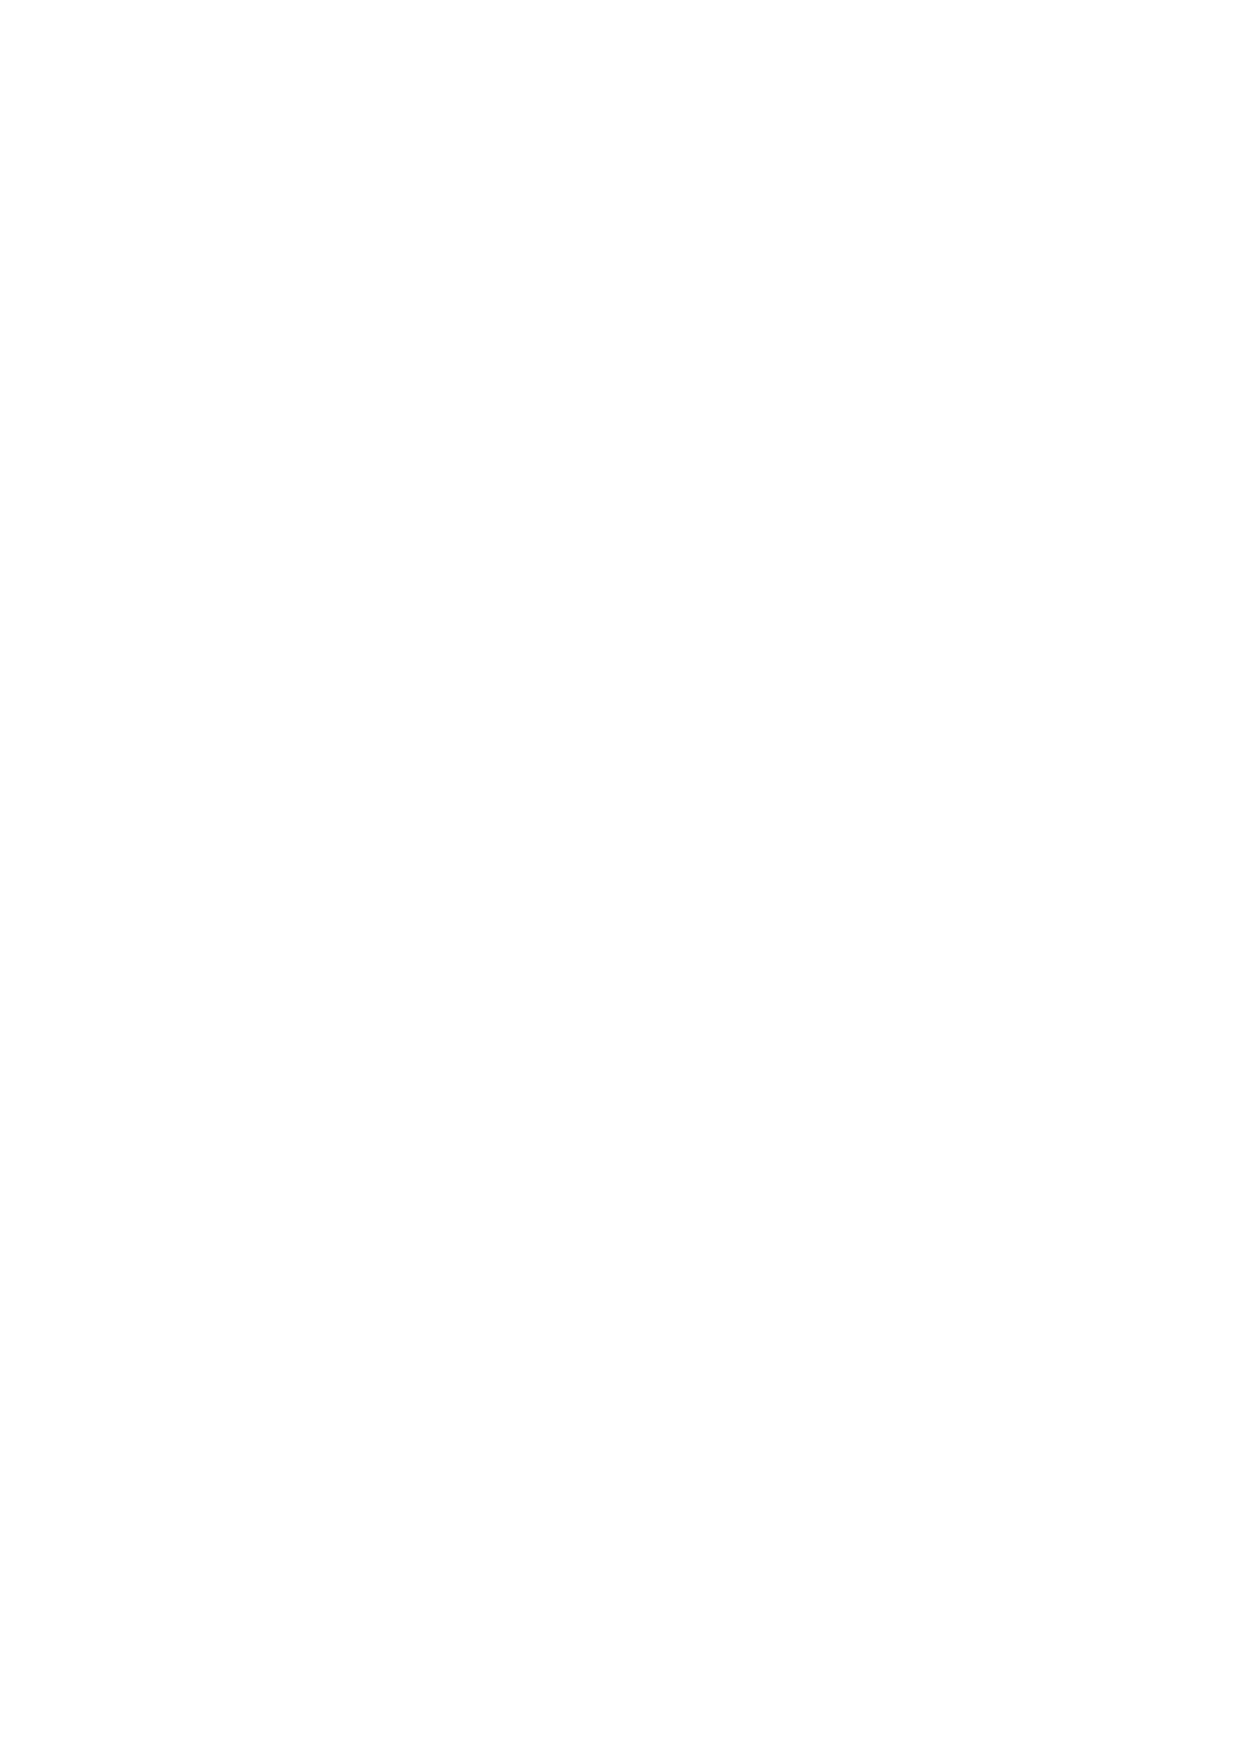
\includegraphics[width=\columnwidth,trim= 0 850 1020 30, clip=true]{./MultimodalDRL/fig/sd}}
\caption{Illustration of Multimodal Architecture and Sensor Dropout. The feature extraction module can be either pure identity function (modality $1$), or convolution-based layer (modality $2 \to M$). The operation $*$ stands for element-wised multiplication.}
\label{fig:Multi-SD}
\end{center}
\end{figure} 

%%% Motivation Effectiveness of Sensor Dropout

% The motivation of Sensor Dropout comes from a potential problem in the sensor-fusion setting. Ideally, we wish that the DRL agent can learn a policy that is not acutely sensitive to any one sensor or a sensor subset. 
% We conjecture that the resulting policy will be more generalized when transferred to other similar tasks, and will also demonstrate robustness to individual sensor noise or even breakdown. In practice, we found out it greatly helps accelerating the policy convergence rate, which indicates that the Sensor Dropout has the potential to operate even in the face of Bellman's curse of dimensionality in the Multi-modal setting.

%%% Implementation : mask and rescale %%%

As shown in Fig.\ref{fig:Multi-SD}, consider the multi-modal state $\tilde{S}$, obtained from feature extraction and given by $\tilde{S}=[\tilde{S}^{(1)}~\tilde{S}^{(2)}~..~\tilde{S}^{(M)}]^T$, where $\tilde{S}^{(i)}= [\tilde{X}_1^{(i)}~\tilde{X}_2^{(i)}~..~\tilde{X}_{K_i}^{(i)}]^T$. 
The objective is to generate a random mask
$\mathbf{c} = [\delta_{c}^{(1)}~\delta_{c}^{(2)}~..~\delta_{c}^{(M)}]^T$, where $\delta_{c}^{(i)} \in \{0,1\}$ represents the on/off indicator for the $i^{th}$ modality.
% $\mathbf{\delta_{c}} = [1^{(1)}~0^{(2)}~..~1^{(K)}]^T$ that switches off a subset of sensors at random. 
However, we need that at least one sensor remains \emph{on} at any given instant in order to maintain training stability. Therefore, we cannot naively extend original dropout idea to sensor blocks $\tilde{S}^{(i)}$.

Let each block's on/off status be sampled from a Bernoulli distribution. We can generate $2^M$ random layer configurations masks and one of them is all the blocks switched off, i.e.,  $\mathbf{{c_0}} = [0^{(1)}~0^{(2)}~..~0^{(M)}]^T$. The probability of this event occurring decreases exponentially in the size of $M$, therefore not having much impact as formulated in \citet{dropout}, where its applied to individual nodes of a layer. However, when $M$ is small as in the case of Sensor Dropout, the probability of $\mathbf{{c_0}}$ occurring is high enough to severely impact training performance. Therefore, we explicitly remove this rogue case and only consider $2^M-1$ layer configuration masks. 
%
Another motivation for Sensor Dropout is to allow for each block $\tilde{S}^{(i)}$ to have a unique dropout probability $p^{(i)}$, if required, with the added cost of more hyper-parameter tuning. However, this tuning is tractable and meaningful in this setup.

%By making the above-mentioned changes and seeking to analyze from a more global standpoint (i.e. checking if one sensor is operating or three sensors are operating, etc.)

Finally, for this work, we slightly depart from \citet{dropout} in modeling our dropout layer. Instead of modeling Dropout as random process where any sensor block $\tilde{S}^{(i)}$ of the layer is switched on/off with a \textit{fix} probability $p$, we propose an alternative view where the random variable is the layer configuration $\mathbf{c}$ itself and not individual block state $\tilde{S}^{(i)}$. Since there are $N = 2^M - 1$ possible states for $\mathbf{c}$, we accordingly sample from an $N$-state categorical distribution. We denote the probability of a layer configuration $\mathbf{{c_j}}$ occurring with $p_j$, where the subscript $j$ ranges from $1$ to $N$. It is easy to derive the corresponding pseudo-Bernoulli\footnote{ We wish to point out that $p^{(i)}$ is pseudo-Bernoulli as we restrict our attention to cases where at least one sensor block is switched on at any given instant in the layer. This implies that, while the switching on of any sensor block $\tilde{S}^{(i)}$ is independent of the other, switching off is not. So the distribution is no longer fully independent.} distribution for switching on a sensor block $\tilde{S}^{(i)}$. Let us denote that as $p^{(i)}$. 
% Define $P_i$ as the sum over all $p^{(i)}$ where $\delta_{c_j}^{(i)} = 1$, i.e. summing over all mask configurations where sensor $\tilde{S}^{(i)}$ is on, as shown below.
% \begin{align}
% P_i = \sum_{j=1}^N\delta_{c_j}^{(i)} p_j \implies P_i \geq 1. 
% \end{align}
% Now, $p^{(i)}$ is nothing but $P_i$ normalized over all $M$ modalities, as shown below.
% \begin{align}
% {p}^{(i)} = \frac{P_i}{\sum_{i=1}^M P_i}
% \end{align}
\begin{align}
{p}^{(i)} = \sum_{j=1}^N\delta_{c_j}^{(i)} p_j
\end{align}
%\textbf{Remark:} %\todo{This para can be made a footnote also, upto you people.} 


Once the sensor dropout mask is applied, we have to deal with the issue of rescaling the non-zero weights. For this, we follow the same convention as in \citet{dropout} but extend it to sensor blocks as opposed to individual nodes. 
\begin{equation}
\alpha_{c_j} = \frac{\sum_{i=1}^M K_i }{\sum_{i=1}^M \delta_{c_j}^{(i)} K_i}.
\end{equation}
% \textit{inversely proportional} to the summation over number of remained hidden units. Denote the dropping configuration as a $K$-element vector $c=[\delta_c^{(1)}~\delta_c^{(2)}~..~\delta_c^{(K)}]^T$, 
% Here, $\delta_{c_j}^{(i)} \in \left\{1,0\right\}$ represent the switching indicator of $i^{th}$ sensor block.
% , the scaling ratio is defined as:
% Note that the scaling ratio is different from the original Dropout \cite{dropout}, which preserved a \textit{neural-wised} constant scaling ratio. Instead, we applied a configuration-dependent scaling which aims to maintain a balanced weighted summation over multiple sensors given different dimensions after feature extraction. It can be interpreted as an approximation of an equally weighted geometric mean of policies suggested by each combination made out of the sensor blocks. 
Finally, the output of Sensor Dropout for the $k^{th}$ node in $i^{th}$ sensor block $\tilde{S}^{(i)}$ for some layer configuration $\mathbf{c_j}$ can be shown as,
\begin{align}
\hat{S}^{(i)}_{{c_j},k} &= \mathcal{M}^{(i)}_{c_j} \tilde{X}_k^{(i)}, \ 
&\text{where} \ \mathcal{M}^{(i)}_{c_j} = \alpha_{c_j} \delta_{c_j}^{(i)}. 
\end{align}
$\mathcal{M}^{(k)}_{c_j}$ is an augmented mask encapsulating both dropout and re-scaling. 

% Intuitively, the combination configurations can be generated from Bernoulli probability, where each sensor block is dropped with $\mathbb{P}(\delta^{(k)}=1) = p_k$. A more generalized form will be Categorical distribution where we explicitly apply heuristics to guide the network perform sensor fusion. These hyper-parameters are problem-specific, and can be pre-defined before training. In this work, we utilize a smaller number of sensor combinations as a proof of concept. The Sensor Dropout is passed by during test time. 

\begin{algorithm}[t]
    \caption{M-DRL with Sensor Dropout}
    \label{alg:mdrl-algo}
\begin{algorithmic}
    \State {\bfseries Input:} Initialize DRL Algorithm \textsc{Agent},\\
    \qquad \quad State pre-processed network $f(\cdot|\theta)$, \\
    \qquad \quad $N$ network configurations $\mathbb{C}= \left\{c_j\right\}_{j=1~..~N}$,\\
    \qquad \quad $N$-state categorical distribution $\mathbb{P}(X=c_j) = p_j$,
    \State Initialize experience replay buffers $\mathcal{B} = \left\{\mathcal{B}_j\right\}_{j=1~..~N}$
    \For{$episode=1$ {\bfseries to} $Eps$ }
     \State Receive initial state $s_1$
     \For{$t=1$ {\bfseries to} $T$}
        \State $\tilde{s}_t \leftarrow f(s_t|\theta)$
        \State $\hat{s}_t \leftarrow$ \textsc{SensorDropout}$(\tilde{s}_t , c_j)$, where $c_j \sim \mathbb{P}$
        \State $a_t \leftarrow $\textsc{Agent.Act}$(\hat{s}_t)$ 
        \State $r_t,s_{t+1},terminate \leftarrow$ \textsc{Env.Observe}$(s_t, a_t)$ 
        \State $\mathcal{B}_j \leftarrow$ \textsc{Query}$(\mathcal{B},c_j)$
        \State $\mathcal{B}_j.$\textsc{Append}$(s_t, a_t, r_t, s_{t+1})$
        \State \textsc{Agent.Update}$(\mathcal{B}_j)$
%        \STATE $t \leftarrow t + 1$
% 	 \UNTIL{$terminate$ is $true$}
     \EndFor
    \EndFor
%    \UNTIL{$t > T_{max}$}
\end{algorithmic}
\end{algorithm}

\subsubsection{Augmenting Experience Replay}
Experience Replay is a commonly used technique in many off-policy DRL algorithms to break the time-based correlation in the agent's experience and thereby stabilize the training process. It differs from the standard deep supervised learning setting, in that batches are sampled from a memory buffer containing all the experience history. However, extending a dropout-like regularization technique to DRL setting to operate on the experience replay is non-trivial and can cause instability because the target values during training are usually non-stationary. In the following paragraph we investigate the instability issue of dropout-like regularization and argue that it is only combinatorially tractable if blocks are dropped out instead of individual nodes. The Sensor Dropout is not only principled but also well-motivated.

First, let us denote an instance of the experience as $[s_{t}, a_{t} , r_{t}, s_{t+1}]$, where $a_{t} = \mu(s_t, \mathcal{\tilde{M}}_{t}) $ is generated from the policy network, with a random mask $\mathcal{\tilde{M}}_{t}$ sampled from an arbitrary distribution at the time step $t$. Note that under the dropout setting, the experience is now \textit{mask configuration dependent}. During Bellman's updates, we calculate the one-step look-ahead target value with $Q^{'}(s_{t+1}, \mu^{'}(s_{t+1},\mathcal{\tilde{M}}_{t+1}))$. 
If two masks, i.e. $\mathcal{\tilde{M}}_{t}$ and $\mathcal{\tilde{M}}_{t+1}$ are not the same, the behavior of $\mu$ and $\mu^{'}$ can be dramatircally different at least in the \textit{beginning of training} as they use different sensor modalities as input and thus causing instability during training.
% Using different masks on $s_t$ and $s_{t+1}$ can make $a_{t}$ and  dramatically different as they may have used different sensor modalities as input and thus causing instability during training.
% This does not happen in supervised learning because we use the true stationary target for training unlike in reinforcement learning where we have a non-stationary target. 
However, under the implementation of Sensor Dropout, this issue can be mitigated by simply maintaining multiple replay buffers for each of the sensor drop configuration $\mathbf{c_j}$. This is not possible with original Dropout as the number of replay buffers will grow exponentially with layer size. Sensor Dropout, on the other hand, makes this tractable as it only grows in the number of sensors. During batch updates, a specific replay buffer is queried given the current layer configuration $\mathbf{c_j}$, followed by the standard batch sampling and update network. This computational advantage makes the principle of sensor-based dropout more attractive and ideally suited in the DRL setting. 

% Moreover, the experience generated at each training step is now \textit{sensor-dropout's configuration dependent}. In order to correctly update the network with experience generated under specific $\mathbf{c_j}$ configuration, one possible way is to maintain multiple replay buffers for each of the sensor drop configuration $\mathbf{c_j}$. This is not possible with Dropout as the number of replay buffers will grow exponentially with layer size. Sensor Dropout, on the other hand, makes this tractable as it only grows in the number of sensors. During batch updates, a specific replay buffer is queried given the current layer configuration $\mathbf{c_j}$, followed by the standard batch sampling and update network. This computational advantage makes the principle of sensor-based dropout more attractive and ideally suited in the DRL setting. 

The overall Multimodal framework with Sensor Dropout regularization is summarized in Algorithm \ref{alg:mdrl-algo}. It can be seen from the above discussion that Sensor Dropout approach is general enough to work with any existing off-policy DRL algorithm in a multi-modal setting. For on-policy algorithms however, Sensor Dropout can be implemented by fixing layer configuration $\mathbf{c_j}$ for every episode. In the next section, we validate the above-mentioned techniques in an open-source racing game called TORCS \cite{wymann2000torcs} and analyze their efficacy.

% \sainote{ I am adding this as explanation for separate replay buffer. (need to make the notations consistent and integrate this to the section)}
% Let say an instance of the experience $[s_{i,t}, a_{i,t} , r_{i,t}, s_{i+1,t}]$, where $a_{i,t}$ is generated using layer configuration $\mathbf{c_j}$, stored in the replay buffer was picked for the bellman update step. During the bellman update step for finding the target, we calculate $Q'(s_{i+1}, \mu'(s_{i+1}))$ where $\mu'(s_{i+1})$-- actor, uses a mask $M_p$. We claim that making sure $M_k = M_p$ improves the training speed and the performance of the agent. This is because although the critic uses the unmasked states, the action is a function of depends on the mask. Using different masks on $s_i$ and $s_{i+1}$ could make $a_{i,t}$ and $\mu(s_{i+1})$ dramatically different as they might have used different sensors as input and thus difficult to learn from. This does not happen in supervised learning because we use the true stationary target for training unlike in reinforcement learning where we have a non-stationary target.

\subsection{Platform Setup} \label{sec:platform}
%%% Define the observation and action %%%
\subsubsection{TORCS Simulator:}
The proposed approach was verified on TORCS \cite{wymann2000torcs}, a popular open-source car racing simulator that is capable of simulating physically realistic vehicle dynamics as well as multiple sensing modalities \cite{GymTORCS} to build sophisticated AI agents. In order to make the learning problem representative of the real-world setting, we picked the following sensors from the TORCS package: the 2D laser range finder, front-view camera with RGB channel, vehicle state - position and speed. % Sensor detail is illustrated in Supplementary. 
The action space is a continuous vector in $\mathbb{R}^3$, whose elements represent acceleration, steering angle, and braking, respectively. Moreover, all the actions are bounded and for this learning problem they are also normalized.

\textbf{Exploration and Reward:} %%%
An exploration strategy is injected adding an Ornstein-Uhlenbeck process noise \cite{uhlenbeck1930theory} to the output of the policy network. 
The choice of reward function is slightly different from  \citet{DBLP:journals/corr/LillicrapHPHETS15} and \citet{A3C} as an additional penalty term to penalize side-ways drifting along the track was added. In practice, this modification leads to more stable policies during training \cite{BenLau16}. % During training, a stochastic process is applied to enforce positive noise on brake angle\cite{BenLau16}. Since stepping on the break naturally violates the reward, such a stochastic process gives the agent a larger exploration probability when a sharp turn is encoutered. \todo{talk about stochastic break or not?} 

\begin{figure}[t]
	\centering
	\begin{subfigure}[b]{0.4\linewidth}
		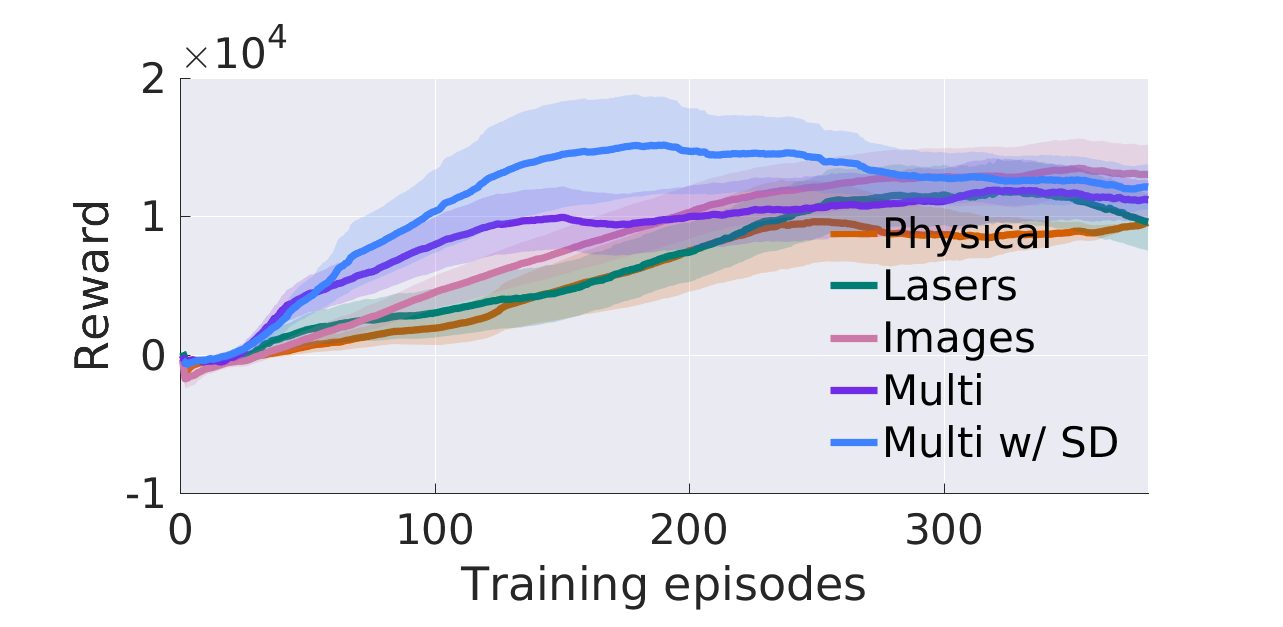
\includegraphics[width=0.9\columnwidth]{./MultimodalDRL/fig/training_exp_naf}
		\subcaption{NAF}
		\label{fig:training_exp_naf}
	\end{subfigure}
	\begin{subfigure}[b]{0.4\linewidth}
		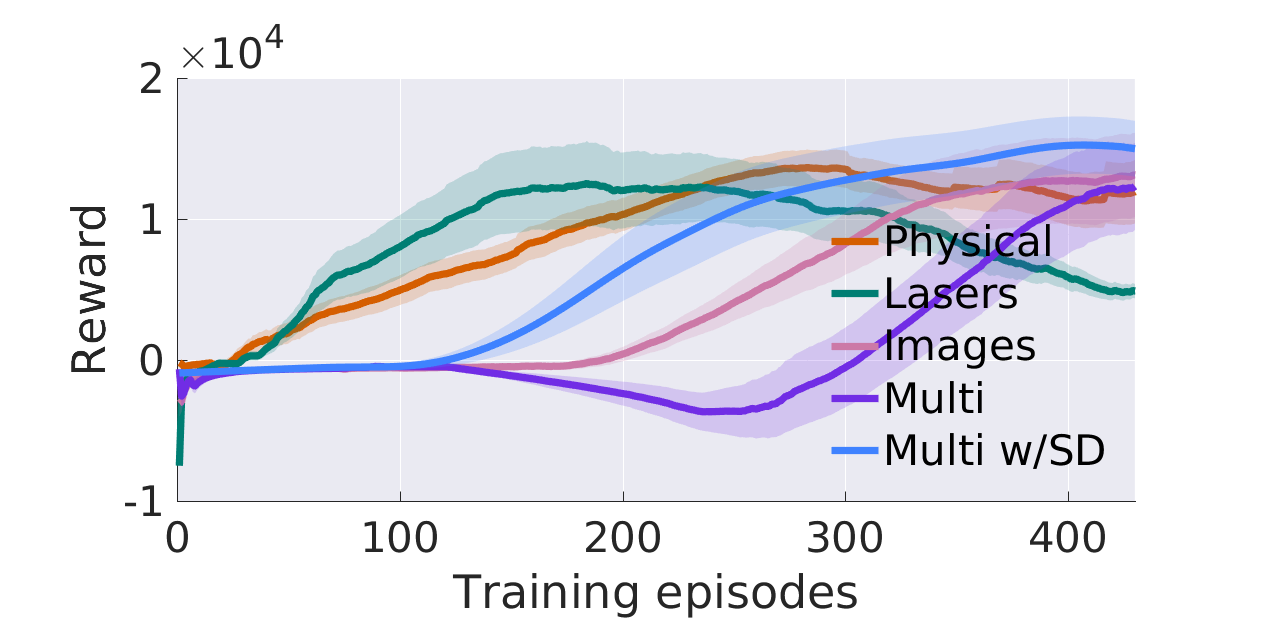
\includegraphics[width=0.9\columnwidth]{./MultimodalDRL/fig/training_exp_ddpg}
		\subcaption{DDPG}
		\label{fig:training_exp_ddpg}
	\end{subfigure}
	\caption{Training performance comparison of three baseline single sensor policies, and the proposed multi-modal policies, with and without Sensor Dropout.}
	\label{fig:training_exp}
\end{figure}

\textbf{State Information:}
% \todo{the minimal representation  in order to maintain the}
Most of the related works use either low-dimensional physical state such as joint angles, or high-dimensional pixels as input. Here, we use the following sensing modalities for our state description: (1) We define \emph{Sensor 1} as a $10$ DOF hybrid state containing all physical information, including $3$D velocity ($3$ DOF), position and orientation with respect to track center-line ($2$ DOF), and finally rotational speed of $4$ wheels ($4$ DOF) and engine ($1$ DOF). (2) \emph{Sensor 2} consists of $4$ consecutive laser scans (i.e., at time $t$, we input scans from times $t,~ t-1,~t-2~\&~t-3$). Here, each laser scan is composed of $19$ readings spanning a $180\degree$ field-of-view in the the front of car. Finally, as \emph{Sensor 3}, we supply $4$ consecutive color images capturing the car's front-view and each one has a resolution $64 \times 64$.

These three representations are used separately to develop our baseline single sensor based policies. The multi-modal state on the other hand has access to all sensors at any given point. When Sensor Dropout (SD) is applied, agent will randomly lose access to a strict subset of sensors. To this end, three different categorical distributions on dropping configurations have been experimented with, and the best learned policy among three configurations is reported here. A more detailed commentary on sensor-fusion configurations follows in Section \ref{sec:SD-config}, with network details listed in the Appendix.

\subsection{Results}
\textbf{Convergence:}
% Note that we remove the result of NAF with image as its input to make it less confusing for comparison. In testing it failed to perform a reasonable policy and ended up with large negative rewards.
The training performance, for all the proposed models and their corresponding baselines, is shown in Fig. \ref{fig:training_exp}. As expected, using high dimensional sensory input directly impacts convergence rate of the policy.
%Sensor Dropout thus played an important role in that instead of searching policy in the entire multi-state space, agent occasionally observed a smaller but still representative states. 
However, despite the curse of dimensionality, the convergence rate improves with the addition of Sensor Dropout, and quite drastically so for DDPG (see Fig. \ref{fig:training_exp_ddpg}).

%We observed that NAF has a much faster convergence rate compared with DDPG. As the fact that value-based method generally performs more efficiently compared with policy-gradient based method, we also related the difference to the actual implementation where additional dense layers were added in between feature extraction modules and NAF agent. More details about this comparison are listed in Section \ref{discussion-NAF}.
To assess the degree of generalization of the learned policies, we pick the the best learned policies for each model and test its performance on other racing tracks. As summarized in Fig. \ref{fig:actual_robust}, we find that the DDPG agent is capable of finding a reasonable policy regardless of the representation of states. The performance of NAF on the other hand is greatly affected by the dimensionality of the agent's input. In fact, the agent fails to achieve even a non-zero reward during testing, when trained with image as input. However, using multi-sensor information and thereby reducing the fused input dimension aids in learning a good policy. Network architecture details are described in Section \ref{discussion-NAF}.

\begin{figure}[t]
	\centering
	\begin{subfigure}[b]{0.4\linewidth}
		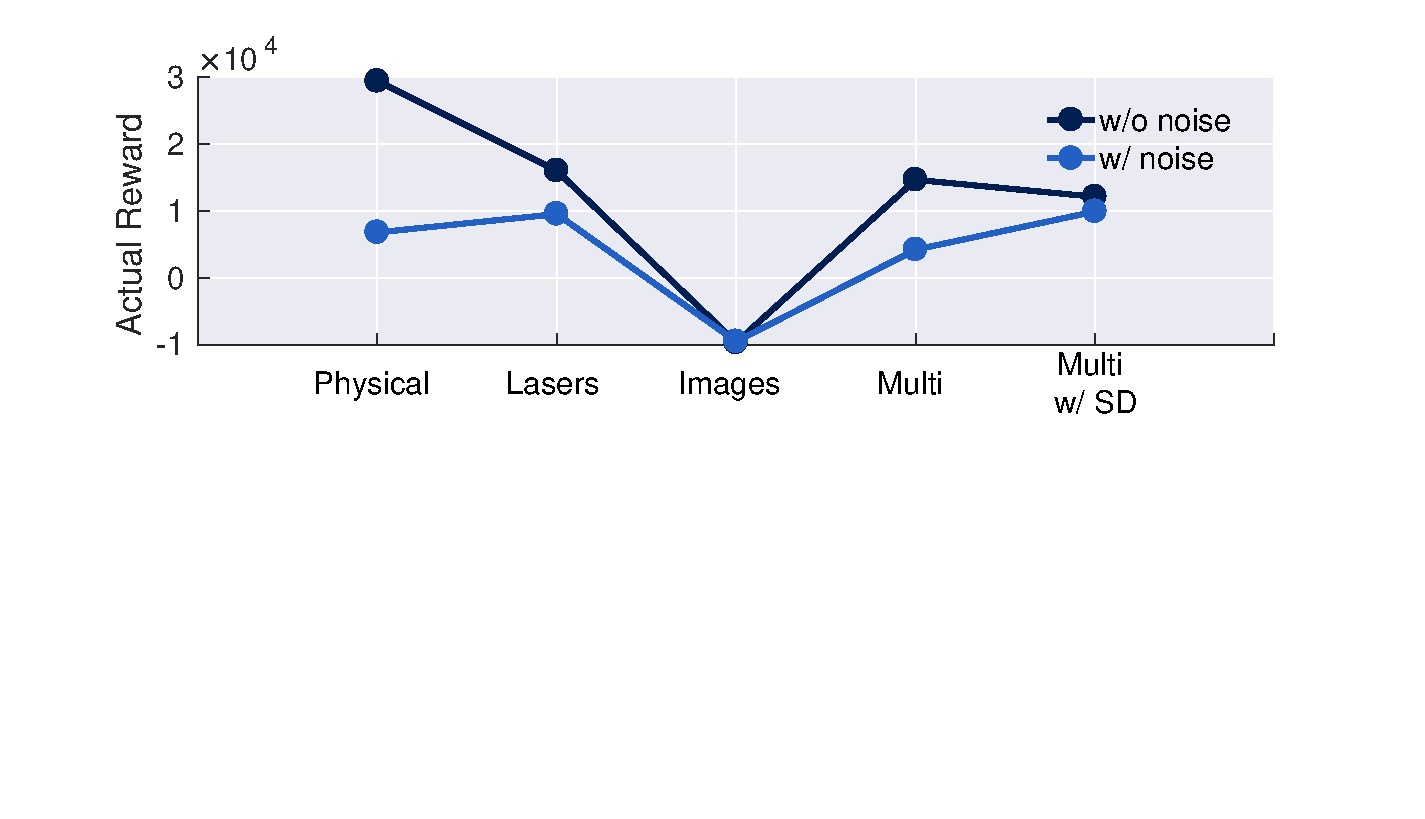
\includegraphics[width=0.9\columnwidth]{./MultimodalDRL/fig/actual_robust_naf}
		\subcaption{NAF}
		\label{fig:actual_robust_naf}
	\end{subfigure}
	\begin{subfigure}[b]{0.4\linewidth}
		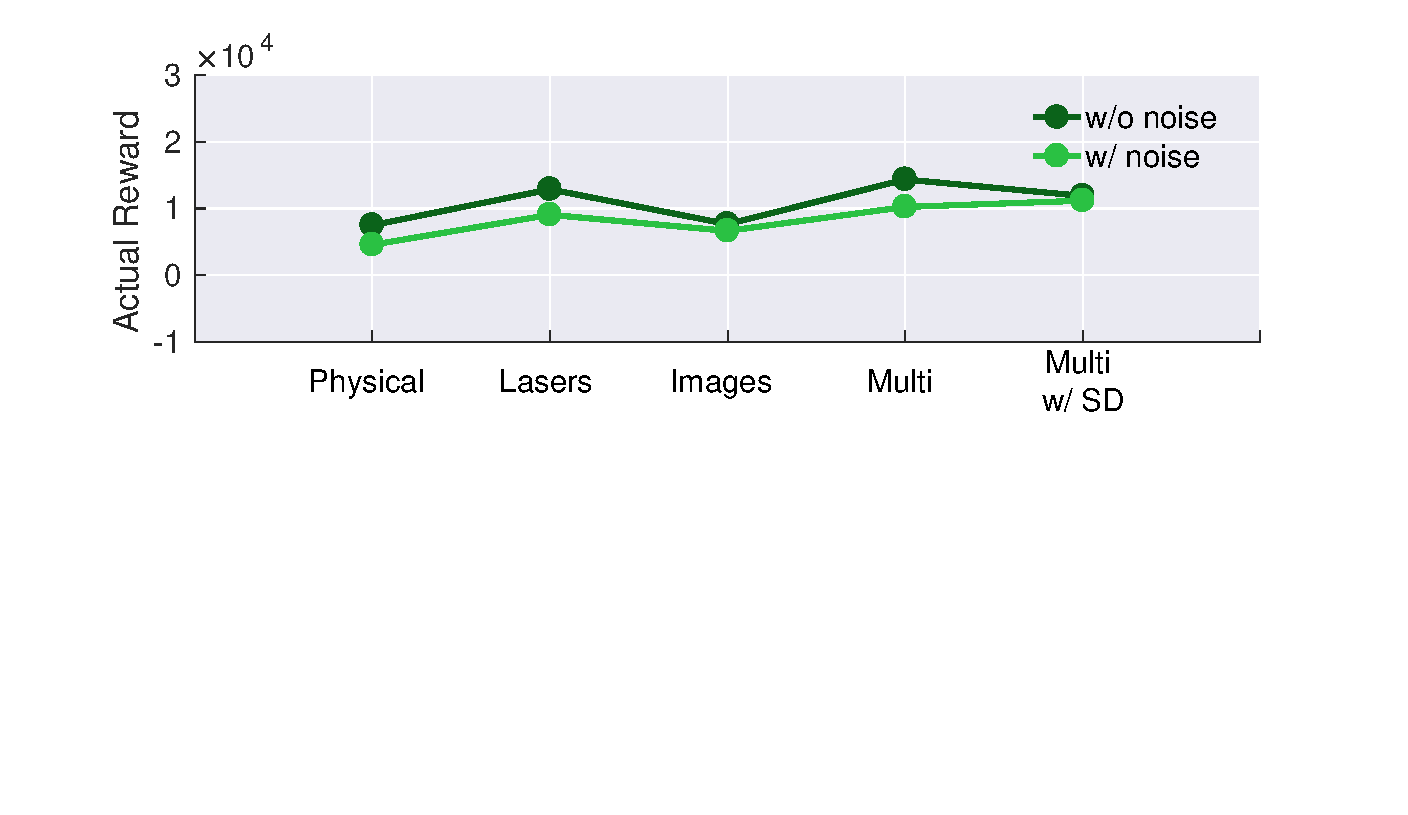
\includegraphics[width=0.9\columnwidth]{./MultimodalDRL/fig/actual_robust_ddpg}
		\subcaption{DDPG}
		\label{fig:actual_robust_ddpg}
	\end{subfigure}
	\caption{Policy Robustness Analysis: Darker lines connects average rewards of leaned policies with accurate sensing while the lighter lines connects the corresponding policies in the face of sensor noise.}
    \label{fig:actual_robust}
\end{figure}

% B. Without Noise experiment % 
% 1. DDPG looks well
% 2. Uni-modal NAF : actual reward decrease proportionally when state dim. increase or state is too abstract.
% -> we claim Multi-modal setting help alleviate the situation
\textbf{Robustness:} Note that, we assumed perfect sensing during the training. However, to test performance in a more realistic scenario, we simulate mildly imperfect sensing by adding gaussian noise. Policy performance with and without noise is plotted for comparison in Fig. \ref{fig:actual_robust}.
% while the relative drop in performance is shown using box-plots in Fig. \ref{fig:relative_robust}.
With the addition of noise the performance drop is sometimes severe in a single input policy, as seen for NAF with physical state input. In comparison, the drop is ore contained for the multi-modal policy and almost negligible when Sensor Dropout is used.

% \begin{figure}[t]
% \centering
% \vskip 0.2in
% \subfigure[NAF]{\label{fig:relative_robust_naf}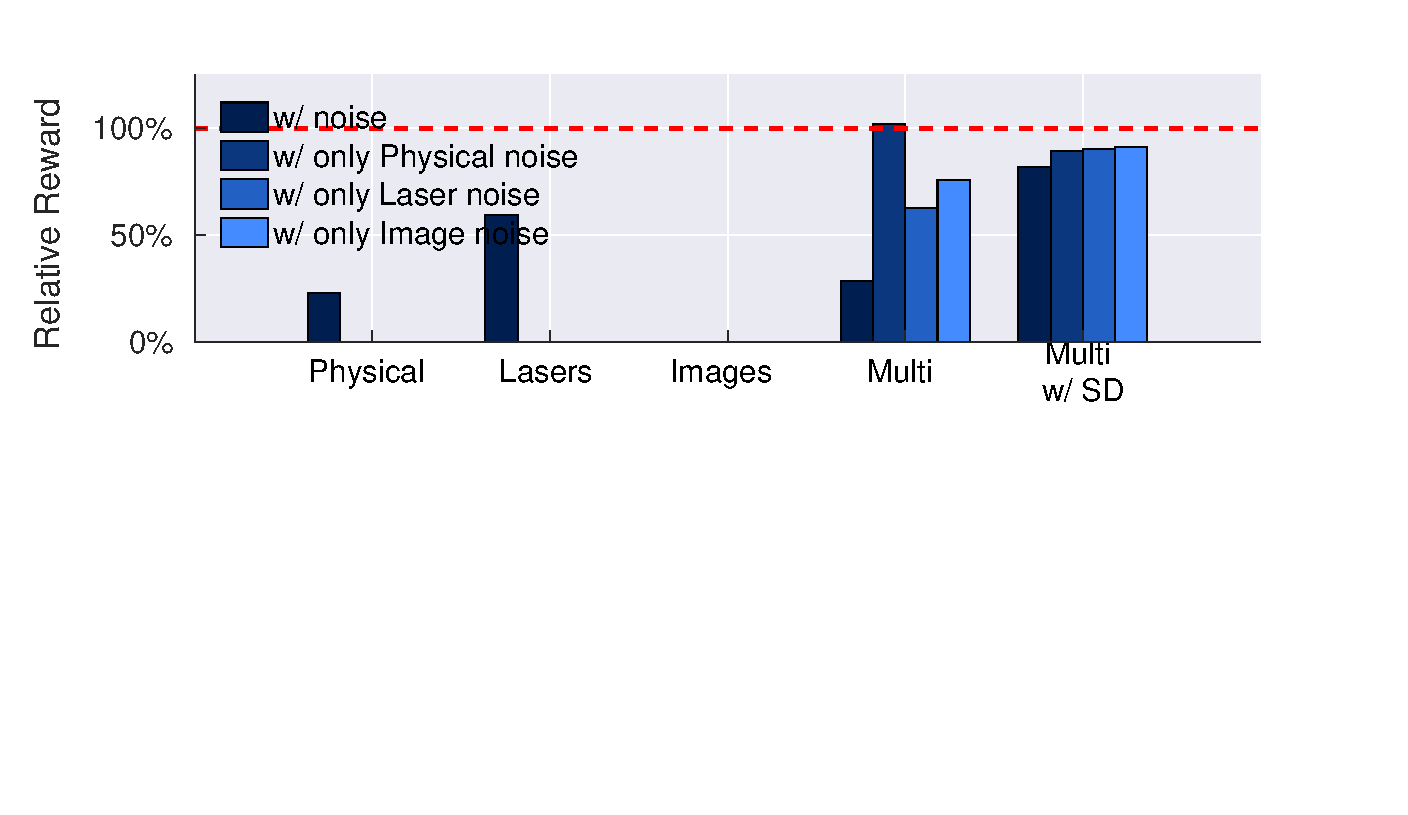
\includegraphics[width=\columnwidth,trim= 0 180 0 25, clip=true]{fig/relative_robust_naf}} % robust_exp_naf
% \subfigure[DDPG]{\label{fig:relative_robust_ddpg}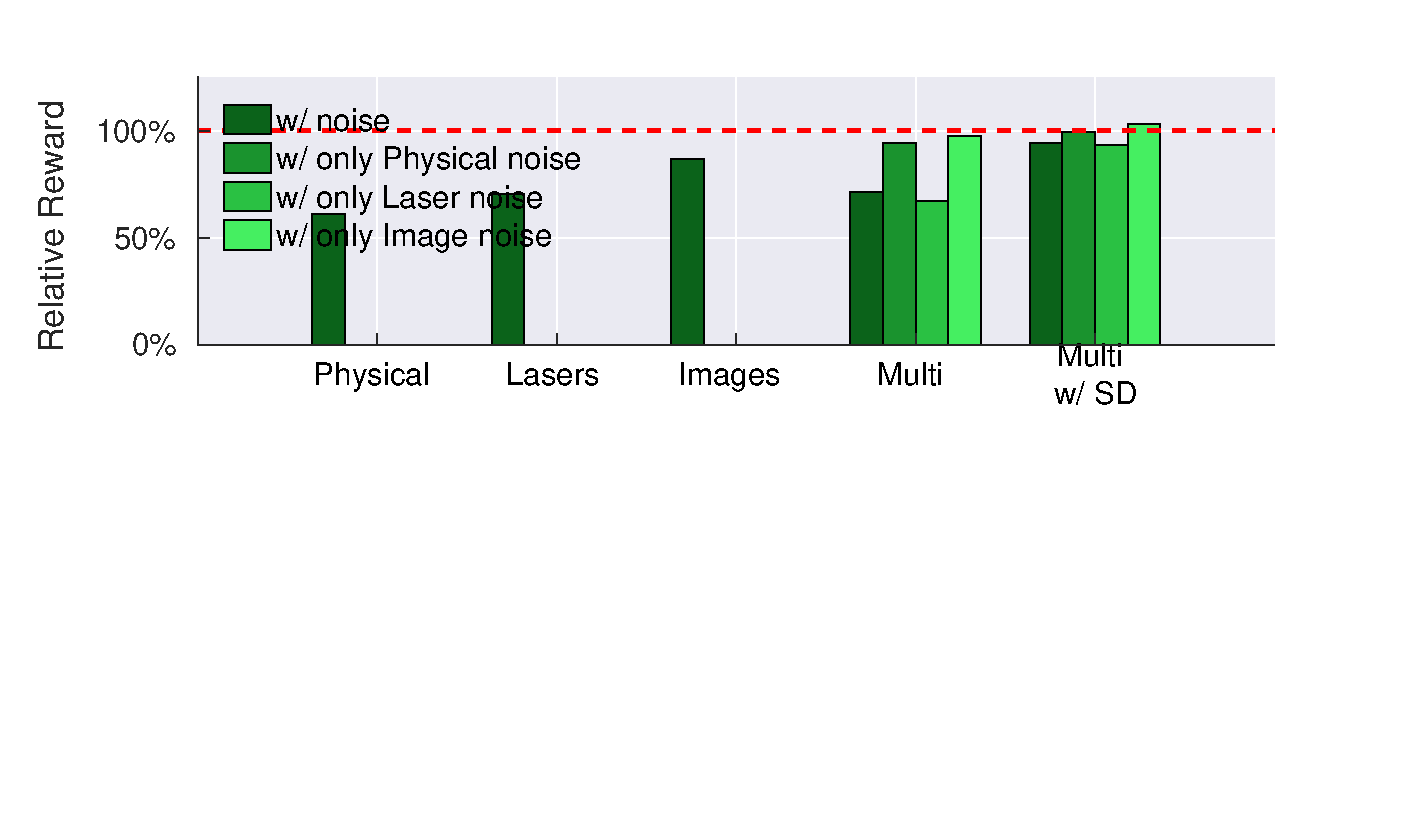
\includegraphics[width=\columnwidth,trim= 0 180 0 25, clip=true]{fig/relative_robust_ddpg}} % robust_exp_ddpg
% \caption{Relative reward of robustness analysis experiment. The bar box measures the relative scale among each of the models when noise is introduced. The red dotted lines show the performance without noise.}
% \label{fig:relative_robust}
% \vskip -0.2in
% \end{figure}

% C. With Noise experiment % 
% 1. NAF perform poorly when noise is introduced. DDPG on the other hand is less sensitive to noise 2. Introducing of SD help both algorithm 
% The perturbation sensitivity is compatible with a more standard Average Fisher Sensitivity (AFS) according to \cite{progressive_net}. The relative performance compared with a noiseless environment is summarized in Fig. \ref{fig:relative_robust}. The performance of the NAF agent drops dramatically when the noise is introduced. From Fig. \ref{fig:training_exp_naf} we also observed that NAF in the multi-modal is sensitive to states from sensors which are easily interpretable such as laser scanners. This effect shows that using an over-complete state representation holds a risk of the agent learning an undesired policy where the influence of different features gets unbalanced. The regularization introduced by Sensor Dropout alleviates this issue and learns a stable policy on both algorithms, with only slight decrease of the performance compared with multi-modal agents trained without SD as shown in Fig. \ref{fig:actual_robust} and \ref{fig:relative_robust}.

\begin{figure}[t]
\begin{center}
\centerline{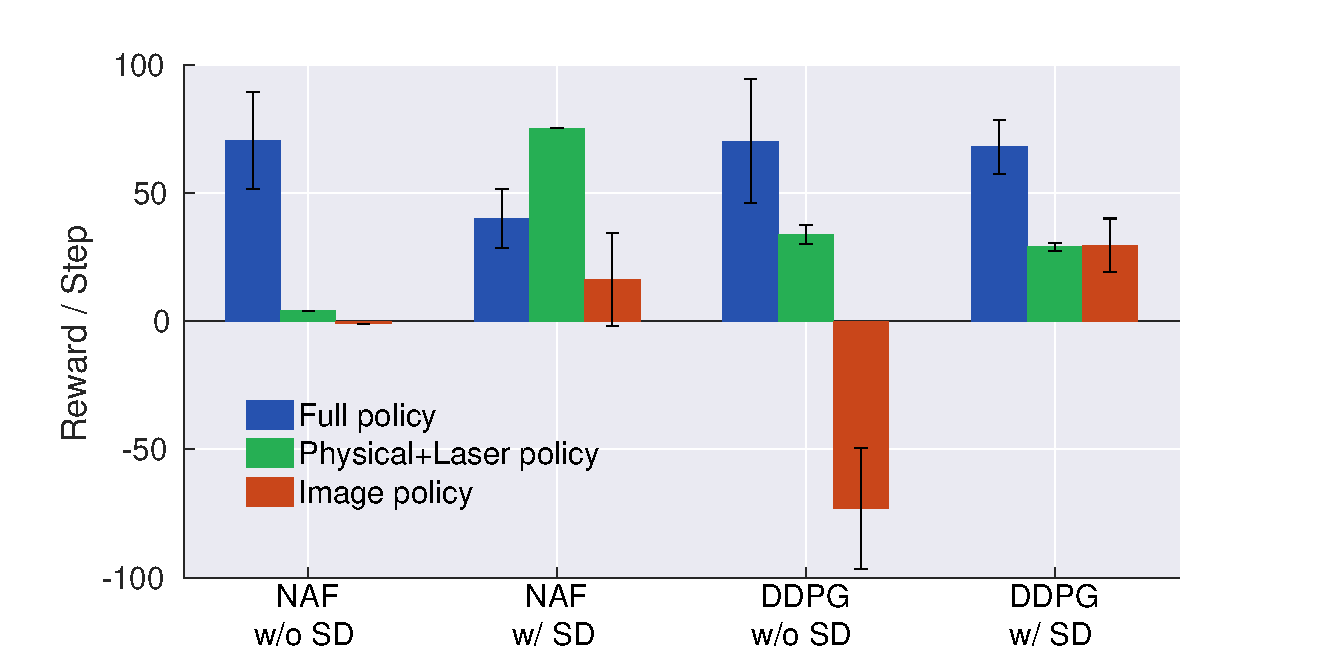
\includegraphics[width=0.9\columnwidth]{./MultimodalDRL/fig/policy}}
\caption{Policy Sensitivity to Sensor Failure: The blue, green, and red bars denote full multi-modal policy, multi-modal with no image input, and multi-modal with no laser and physical state input, respectively.}
\label{fig:policy_exp}
\end{center}
\end{figure} 

\textbf{Sensitivity Analysis:} \label{sec:policy}
% Best policy analysis
In this part, we further validate our hypothesis Sensor Dropout (SD) reduces the learned policy's acute dependence on a subset of sensors in a multi-modal setting. First, we considered a scenario when malfunction of a sensor has been detected by the system, and the agent need to rely on the remaining sensors to make the decision. During testing, we manually blocked off part of the sensor modules, and scaled the rest of observation using the same rescaling mechanism as proposed in Section \ref{sec:SD}. Fig. \ref{fig:policy_exp} reports the average of the normalized reward, i.e. total reward divided by total steps, of each model. For both the algorithms, models trained with SD performed comparatively better when decisions were forced to depend on a subset of sensors than the ones trained without SD. We observed that the policy could either be highly correlated, which is the case of NAF w/o SD in Fig. \ref{fig:policy_exp}, or depend on sensor subset, as shown in DDPG w/o SD in Fig. \ref{fig:policy_exp}. We therefore emphasize that introducing Sensor Dropout during training has significant practical benefits, in that the policies induced by different configurations of sensors are learned at the same time. 
% Moreover, using SD will lead to robust feature extraction modules when network being joint optimized since all policies share the same variables in the \textit{back-end} DRL agent.

\subsection{Probing through the gradients}

\begin{table}[t]
\begin{center}
% \captionsetup{justification=centering}
\caption{Results of the $\mathcal{T}_2^1$ dependency metric.}
\label{table:policy-ratio}
\begin{small}
% \begin{sc}
% \begin{tabular}{@{}cccccc@{}}
\begin{tabular}{cccccc}
\toprule 
\centering
 & & \multicolumn{2}{c}{Training Env.} & \multicolumn{2}{c}{Testing Env.}  \\
 & & Mean & Median & Mean & Median \\ \midrule \midrule
\multirow{2}{*}{NAF}  & w/o SD & 1.651 & 1.871 & 1.722 & 1.940 \\
                      & w/ SD  & \textbf{1.284} & \textbf{1.379} & \textbf{1.086} & \textbf{1.112} \\ \midrule
\multirow{2}{*}{DDPG} & w/o SD & 1.458 & 1.449 & 1.468 & 1.437 \\
                      & w/ SD  & \textbf{1.168} & \textbf{1.072} & \textbf{1.171} & \textbf{1.120} \\ \toprule
\end{tabular}
% \end{sc}
\end{small}
\end{center}
\end{table}

\subsubsection{Dependency metric:}
To further examine the impact of Sensor Dropout on effective sensor fusion, we introduce an intuitive method for monitoring the extent to which the learned policy depends on each sensor block by measuring the gradient of the policy output w.r.t a subset block $\tilde{S}^{(i)}$. In a multi-input-to-output mapping, this denotes the relative weights/importance of each input 
% (in this case the sensor block $\tilde{S}^{(i)}$\todo{duplicate?}). 
Since in this work, SD was implemented to drop either (1) $(physical~state,~ laser)$ or (2) $vision$, we define the \emph{dependency} metric for this problem as the ratio between configurations (1) and (2), as shown below.  
\begin{equation}
\mathcal{T}_2^1 = \frac{1}{M}\sum_{i=1}^M \frac{\left| \nabla_{\tilde{S}^{(1)}_i} \mu (\tilde{S} | \theta^\mu )\Big|_{S_i} \right|}{\left| \nabla_{\tilde{S}^{(2)}_i} \mu (\tilde{S} | \theta^\mu )\Big|_{S_i} \right|} 
\label{equ:grad_metric}
\end{equation}
 Assuming the fusion-of-interest is between the above-mentioned two subsets, we intend to show that, using SD, the metric should get closer to one, indicating nearly equal importance to both the sensing modalities. This metric is evaluated for policies learned with and without SD for NAF and DDPG and the mean values are reported in Table \ref{table:policy-ratio}. For this, the data was collected from a stable policy by evaluating it on both training and testing environments. We can verify that, using SD, NAF policies become dramatically more dependent all sensors. Additionally, we visualize the dependence on each neuron by estimating the average gradient. As shown in Fig. \ref{fig:grad_exp}, models trained with SD tend to make better use of visual information (location is indicated by the red bar.). Without SD however, agents tend to rely more heavily on physical state and laser inputs. 

\begin{figure}[t]
\begin{center}
\centerline{\includegraphics[width=\columnwidth]{./MultimodalDRL/fig/grad2.png}}
\caption{The visualization of the magnitude of gradient for each neuron on training environment. The whiter color means the higher gradient. The color bar represents three different sensor modules: physical state(blue), Laser(green), and Image(red).}
\label{fig:grad_exp}
\end{center}
\end{figure} 

\subsubsection{Visualizing weights:}
% Gradients  part among each sensor the policy net pays more attention to \cite{simonyan2014very}. 
As shown in Fig. \ref{fig:grad_exp}, we observe that models trained with SD have higher gradients on neurons corresponding to the corner inputs of the laser sensor, indicating that a more sparse and meaningful policy is learned. These corner inputs corresponded to the laser beams that are oriented perpendicularly to the vehicle's direction of motion, and give an estimate of its relative position on the track. Clearly, the network is able to automatically infer and weight locations providing salient information. This behavior is consistent in both DDPG and NAF.

To look for similar patterns, in Fig. \ref{fig:grad_exp_img}, image pixels with higher gradients are marked to visualize and interpret the policy's view of the world. We pick two scenarios, 1) straight track and 2) sharp left turn, depicted by the first and second rows in the figure. Models trained with SD tend to capture relevant visual information such as road boundary. In comparisons, models trained without SD have a relatively low and unclear gradients over both laser and image sensor state space.

\begin{figure}[t]
\begin{center}
\centerline{\includegraphics[width=\columnwidth]{./MultimodalDRL/fig/grad_image.png}}
\caption{The gradient responses of actions on the image input for each of the multi-modal agents. The top $20\%$ gradients are marked red.}
\label{fig:grad_exp_img}
\end{center}
\end{figure} 


\section{Discussion}
\subsection{Sensor Dropout v/s \emph{traditional} Dropout}
%%% talk more about some detailed in SD compared with Dropout %%%
In addition to demonstrating the value of using Sensor Dropout, it also critical to verify whether similar performance can be extracted with Dropout or not. Therefore, we implemented the Dropout on our multi-modal agent with dropping probabilities of $0.5$ and $0.25$ as baselines. Both models performed poorly in the testing environment, even with perfect sensing. For DDPG, mean reward using dropout was only $2.2\times 10^3$, compared with $1.1\times 10^4$ and $1.4\times 10^4$, obtained on vanilla-multi-modal policy and multi-modal + SD, respectively. Similar results were observed with NAF too. This furthers our claim that traditional implementation of dropout increases the risk of destabilizing the DRL policy.

\subsection{Fusion Layer Configurations} \label{sec:SD-config}

%%% Setting of SD used in this work %%%

Under the current implementation, the agent will observe the sensor data from one of the following three combinations during training: (1)$(physical~state,~laser)$, (2) $(image)$, or (3) $(physical~state,~laser,~image)$ . 
% As mentioned in Section \ref{sec:SD}, the categorical distribution of these three combinations can be set as hyper-parameters.
We have experimented with following three different settings:(a) $[p_1~p_2] = [0.25~0.25]$, (b) $[p_1~p_2] = [0.4~0.4]$, or (c) $[p_1~p_2] = [0.5~0.5]$. Here, $p_1$ and $p_2$ represent the probability of using the first and second combinations, respectively, while the probability of the third combination $p_3$ is given by $p_3 = 1 - p_1 - p_2$. For the first two configurations, the agent has access to all sensors occasionally, but in the last case, the agent only has access to a subset of sensors at any given point. 

%%% talk more about some detailed in SD compared with Dropout %%%
% 1. training speed (Fast: 0.5 > 0.4 > 0.25 )
% 2. performance in both training/testing (Higher: 0.5 < 0.4 < 0.25 )
% 3. Individual policy (Higher: 0.5 < 0.4 < 0.25 )

We note that as the probabilities $p_1,~p_2$ increase, the policy convergence rate and the normalized average rewards induced by each sensor subset also increase, as described in Section \ref{sec:policy}. However, the performance of the full policy decreases in both training and testing environment. This empirical result suggests a more principled way to apply Sensor Dropout. For instance, we can start with a high value for $(p_1,~p_2)$ and benefit from faster policy convergence for each sensor subset and then gradually decrease the probability to promote fusion. 
% Another practical insight is to apply Sensor Dropout as a prior among failure probability of each sensor subset. 
% Though in practice the difference on performance is almost negligible and won't affect our experiment result, 
\subsection{Implementation of NAF with Multi-modal} \label{discussion-NAF}
Since NAF is not designed for high-dimensional state space, unstable policies result if extended naively to operate with image as input. To mitigate this problem, we add two additional fully-connected layers to reduce the state dimensionality to apply the NAF algorithm. We consider this slight modification as a useful and practical method to embed a low-dimensional representation of visual information. However, purely image-based policy learned with the NAF agent still results in an unstable behavior with large negative rewards \emph{during testing}. This could be a case of over-fitting where the experience from training environment does not generalize well to fully operate in the state space, and the agent may have just memorized specific but irrelevant visual cues. Surprisingly, the multi-modal representation alleviated the issue by fusing visual state with other sensory information. The results specific to NAF and the above-mentioned findings alone offer great scope for greater probing and is saved for future work.

\section{Conclusions and Future Work}
In this work, we extend popular DRL algorithms like DDPG and NAF to the multi-modal setting. Additionally, we introduce a new stochastic regularization technique called Sensor Dropout to promote an effective fusing of information from multiple sensors. 

% Through extensive empirical testing we show the following exciting results,
% \begin{enumerate}
% \item Multimodal-DRL with Sensor Dropout(SD) reduces performance drop in a noisy environment from $\approx 30\%$ to just $5\%$, when compared to a baseline single sensor system.
% \item Policies learned using SD best leverage the multi-modal setting by greatly reducing over-dependence on any one sensing modality. Additionally, for each sensor it was observed that SD enforces sparsity and promotes each sensor to base the policy primarily on intuitive and salient features.
% \item A multi-modal policy with SD guarantees functionality even in a face a sensor failure. This is a huge plus and the best use-case for the need for redundancy in safety-critical application like autonomous navigation.
% \end{enumerate}

For future work, we wish to extend Multi-modal DRL to other algorithms like ICNN \cite{amos2016input}, TRPO \cite{TRPO}, GPS \cite{levine2013guided}, and Q-Prop \cite{DBLP:journals/corr/GuLGTL16}, etc. Secondly, we wish to augment the reward function to also perform other important driving tasks like collision avoidance, and lane changing, etc. Moreover, systematic investigation into the failures of image-based NAF policies and the choices for $p_1 and p_2$ (hyperparameter optimization) are also interesting avenues that merit further study.

\end{document}